\documentclass{article}
\usepackage[scale=.9]{geometry}
\usepackage{tikz}
\usetikzlibrary{knots,hobby,external}

\tikzset{
  external/figure name=knot,
  external/prefix=knotdiagrams/,
}

\tikzexternalize

\let\origtikzsetnextfilename\tikzsetnextfilename
\def\tikzsetnextfilename#1{%
  \origtikzsetnextfilename{#1}%
  \mysetlabel{#1}%
}

\newcommand{\mysetlabel}[1]{%
  \gdef\mynextlabel{#1}}

\newcommand{\autolabel}{%
  \label{fig:\mynextlabel}
  \global\let\mynextlabel\relax
}


\tikzset{
  use Hobby shortcut,
  knot diagram/every strand/.append style={
    ultra thick,red
  },
  every picture/.style={
    execute at end picture={%
      \path ([shift={(-5pt,-5pt)}]current bounding box.south west)   ([shift={(5pt,5pt)}]current bounding box.north east);
    }
  }
}

\begin{document}
%\tikzset{external/force remake=true}
\begin{figure}
\tikzsetnextfilename{unknot}
\centering
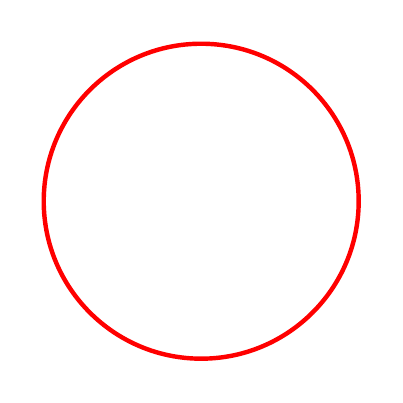
\begin{tikzpicture}
\draw[ultra thick,red] (0,0) circle[radius=2cm];
\end{tikzpicture}
\caption{Unknot}
\autolabel
\end{figure}

\begin{figure}
%% Trefoil
\tikzsetnextfilename{trefoil}
\centering
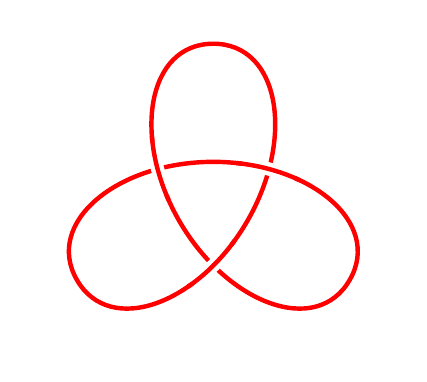
\begin{tikzpicture}
\begin{knot}[
  consider self intersections=true,
%  draft mode=crossings,
  flip crossing=2
  ]
\strand ([closed]90:2) foreach \k in {1,...,3} { .. (-30+\k*240:.5) .. (90+\k*240:2) } (90:2);
\end{knot}
\end{tikzpicture}
\caption{Trefoil}
\autolabel
\end{figure}

\begin{figure}
%% Figure 8
\tikzsetnextfilename{figure8}
%\tikzset{external/export next=false}
\centering
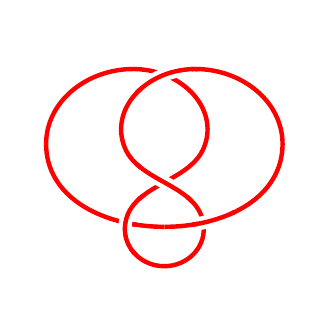
\begin{tikzpicture}
\begin{knot}[
  consider self intersections=true,
%  draft mode=crossings,
  ignore endpoint intersections=false,
  flip crossing=3
]
\strand ([closed]0,0) .. (1.5,1) .. (.5,2) .. (-.5,1) .. (.5,0) .. (0,-.5) .. (-.5,0) .. (.5,1) .. (-.5,2) .. (-1.5,1) .. (0,0);
\end{knot}
\path (0,-.7);
\end{tikzpicture}
\caption{Figure 8}
\autolabel
\end{figure}

\begin{figure}
%% Cinquefoil
\centering
\tikzsetnextfilename{cinquefoil}
%\tikzset{external/export next=false}
%\tikzset{external/force remake}
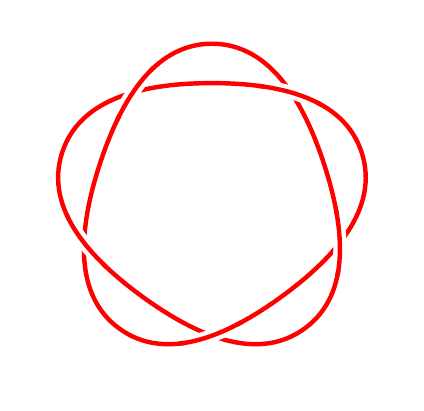
\begin{tikzpicture}
\begin{knot}[
  consider self intersections=true,
%  draft mode=crossings,
  flip crossing/.list={2,4}
  ]
\strand ([closed]90:2) foreach \k in {1,...,5} { .. (18+\k*144:1.5) .. (90+\k*144:2) } (90:2);
\end{knot}
\end{tikzpicture}
\caption{Cinquefoil}
\autolabel
\end{figure}

\begin{figure}
%% 5_2
\centering
\tikzsetnextfilename{5-2}
%\tikzset{external/export next=false}
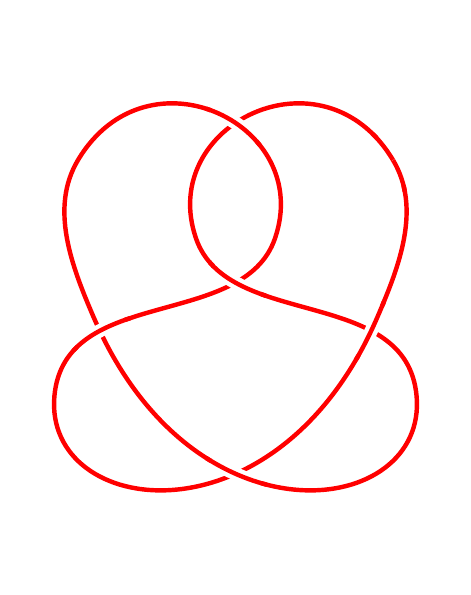
\begin{tikzpicture}
\begin{knot}[
  consider self intersections=true,
%  draft mode=crossings,
  ignore endpoint intersections=false,
  flip crossing/.list={6,4,2}
  ]
\strand ([closed]2,2) .. (1.8,0) .. (-2.3,-1) .. (.5,1) .. (-2,2) .. (-1.8,0) .. (2.3,-1) .. (-.5,1) .. (2,2);
\end{knot}
\end{tikzpicture}
\caption{\(5_2\)}
\autolabel
\end{figure}

\begin{figure}
%% 6_1
\centering
\tikzsetnextfilename{6-1}
%\tikzset{external/export next=false}
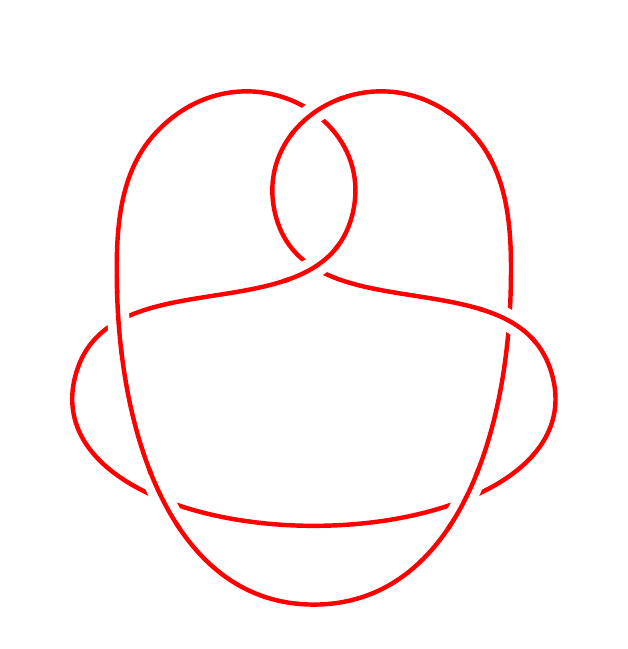
\begin{tikzpicture}
\begin{knot}[
  consider self intersections=true,
%  draft mode=crossings,
  ignore endpoint intersections=false,
  flip crossing/.list={7,4,2},
  clip width=5,
  ]
\strand ([closed]2,2) .. (2.5,0) .. (0,-4) .. (-2.5,0) .. (-2,2) .. (.5,1) .. (-3,-1) .. (0,-3) .. (3,-1) .. (-.5,1) .. (2,2);
\end{knot}
\end{tikzpicture}
\caption{\(6_1\)}
\autolabel
\end{figure}

\begin{figure}
%% 6_2
\centering
\tikzsetnextfilename{6-2}
%\tikzset{external/export next=false}
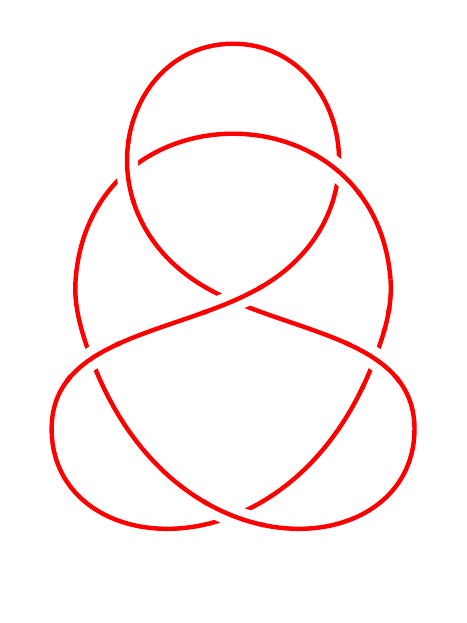
\begin{tikzpicture}
\begin{knot}[
  consider self intersections=true,
%  draft mode=crossings,
  ignore endpoint intersections=false,
  flip crossing/.list={9,5,4},
  clip width=5,
  ]
\strand ([closed]2,1) .. (1.8,0) .. (-2.3,-1) .. (.5,1) .. (0,4) .. (-.5,1) .. (2.3,-1) .. (-1.8,0) .. (-2,1) .. (2,1);
\end{knot}
\end{tikzpicture}
\caption{\(6_2\)}
\autolabel
\end{figure}

\begin{figure}
%% 6_3
\centering
\tikzsetnextfilename{6-3}
%\tikzset{external/export next=false}
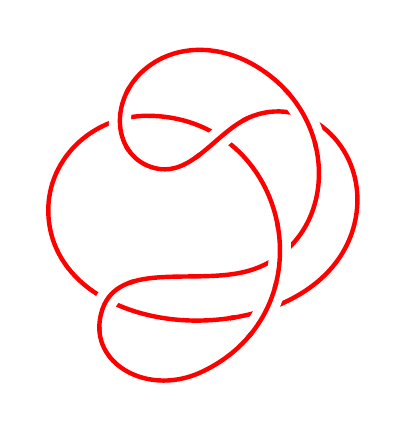
\begin{tikzpicture}
\begin{knot}[
  consider self intersections=true,
%  draft mode=crossings,
  ignore endpoint intersections=false,
  flip crossing/.list={7,1,4},
  clip width=5
  ]
\strand[scale=1.3] ([closed]0,0) .. (1.5,1) .. (.5,2) .. (-.5,1.5) .. (-.5,2.5) .. (.5,2.5) .. (.5,.5) .. (-1,0) .. (0,-.5) .. (-.5,2) .. (-1.5,1) .. (0,0);
\end{knot}
\end{tikzpicture}
\caption{\(6_3\)}
\autolabel
\end{figure}

\begin{figure}
%% 7_1
\centering
\tikzsetnextfilename{7-1}
%\tikzset{external/export next=false}
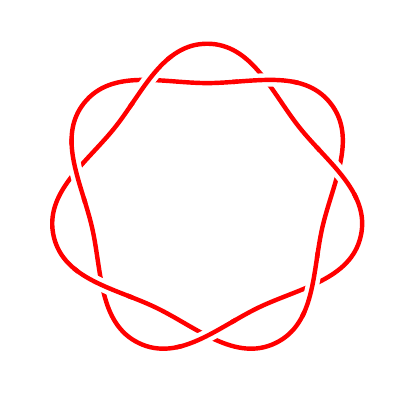
\begin{tikzpicture}
\begin{knot}[
  consider self intersections=true,
%  draft mode=crossings,
  flip crossing/.list={2,4,6}
]
\strand ([closed]90:2) foreach \k in {1,...,7} { .. (90-360/7+\k*720/7:1.5) .. (90+\k*720/7:2) } (90:2);
\end{knot}
\end{tikzpicture}
\caption{\(7_1\)}
\autolabel
\end{figure}

\begin{figure}
%% 7_2
\centering
\tikzsetnextfilename{7-2}
\tikzset{external/export next=false}
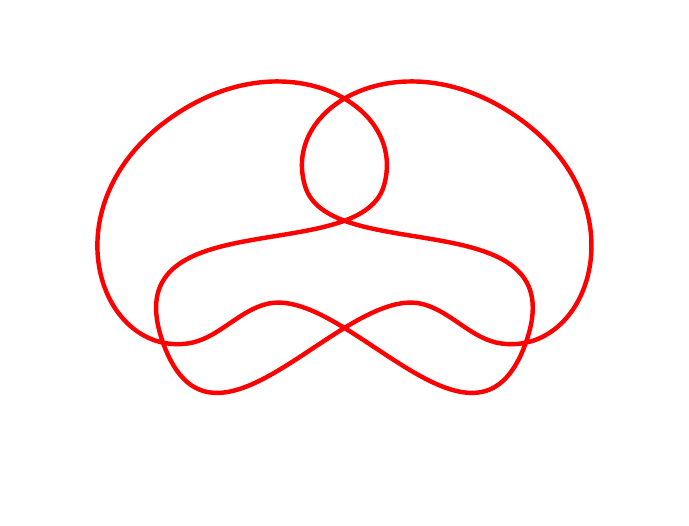
\begin{tikzpicture}
\begin{knot}[
]
\strand ([closed]2,2) .. (2,-1) .. (1,-.5) .. (-2.3,-1) .. (.5,1) .. (-2,2) .. (-2,-1) .. (-1,-.5) .. (2.3,-1) .. (-.5,1) .. (2,2);
\end{knot}
\end{tikzpicture}
\caption{\(7_2\)}
\autolabel
\end{figure}
\end{document}
